\documentclass[12pt, letterpaper]{article}
\usepackage{graphicx} % Required for inserting images

\title{Senior Design Manual}
\author{Bennett Petzold, Holly Grant, Hunter Marlette, Patrick Burke}
\date{Version 0.1 - April 2023}

% Formatting
\usepackage[left=0.5in, right=0.5in, top=1in, bottom=1in, letterpaper]{geometry}
\usepackage{kpfonts} % https://r2src.github.io/top10fonts/
\usepackage{microtype} % Makes the formatting look nicer
\usepackage{graphicx} % Graphics: https://www.overleaf.com/learn/latex/Inserting_Images
\graphicspath{{./graphics}}
\usepackage{caption} % Image captions
\usepackage{indentfirst} % Indent the first paragraph of a section
\usepackage{booktabs}
\usepackage{tabularx}
\usepackage{array}
\usepackage[indent]{parskip}

% Utility
\usepackage{hyperref} % Hyperlinks
\usepackage[nameinlink]{cleveref} % Improved refs
\crefformat{figure}{[#2fig. #1#3]}
\usepackage{changepage} % Text body indent adjustment
\usepackage{enotez} % Footnotes at end of document
\setenotez{list-name=, backref=true}
\usepackage{minted} % Code formatting
\setmintedinline{breaklines}

\usepackage{xcolor} % used to highlight text
\usepackage{soul} % used for \hl{} command 

\usepackage{caption}
\usepackage{subcaption}

%\usepackage{enumerate}
%\usepackage{enumitem}
%\usepackage[english]{babel}

% Hyperref setup
\hypersetup{
    colorlinks=true,
    linkcolor=blue,
    filecolor=magenta,      
    urlcolor=red,
    pdftitle={Overleaf Example},
    pdfpagemode=FullScreen
}

% Combine href with a footnote link
\newcommand\lref[2]{
    \href{#1}{#2}%
    \endnote{\href{#1}{#1}}%
}

% Environment with subsubsection and its contents indented
% Need this fix... don't ask me why: https://tex.stackexchange.com/a/65865
\newcommand{\subsub}[1]{ {\begin{adjustwidth}{3em}{0pt} \nointerlineskip\leavevmode \subsubsection{#1} \end{adjustwidth}} }
\newenvironment{subsubsec}[1]{\begin{adjustwidth}{2cm}{} \nointerlineskip\leavevmode \subsubsection{#1}}{\end{adjustwidth}}
% Adjusting table of contents indenting
%\usepackage{titletoc,tocloft}
%\setlength{\cftsubsecindent}{1cm} % Subsection indent
%\setlength{\cftsubsubsecindent}{2cm} % Subsubsection indent

% Misc. shorthands
\newcommand{\bashline}[1]{\textbf{\mintinline{bash}{#1}}}

\begin{document}

\maketitle

%\hl{\textbf{NOTE: }Highlighted text like this note means that there is something that needs to be edited, replaced, or added at this section and should is not finalized!}

\tableofcontents{}
\pagebreak{}

\section{Introduction}
The ECE MakerSpace requires training for specific devices with complex or potentially dangerous methods of operation but has no way of enforcing this rule and preventing unauthorized users from accessing those devices. This device was designed to monitor and restrict that access while logging the data associated with each use of every device.

\section{Bill of Materials}
% BOM table formatting
\newcolumntype{I}{m{0.45\textwidth}}
\newcolumntype{Q}{>{\centering\arraybackslash}m{0.075\textwidth}}
\newcolumntype{L}{m{0.25\textwidth}}
\newenvironment{bomTable}
    { \begin{center}
        \setlength{\tabcolsep}{24pt}
        \begin{tabular}{@{\hspace{2em}} I Q L @{}} }
    { \end{tabular}\end{center} \vspace{1em} }

%\hl{Part numbers and order information can be found in the Senior Design Order form document.}

%\hl{Add part numbers to this part of the documentation (instead of links?!) }
Full BOM and cost breakdown can be found \lref{https://docs.google.com/spreadsheets/d/1I3pgFnPUj8xgdaECBA7j94ydT4JwhcCwujzxo4dt6PY/edit\#gid=97521878}{here}.\\

\subsection{Main Components}
%\hl {\textbf{Note: }Asterisks where the link needs to be (*********) means that I either need to find the link or do not have the link currently. There should be none of these in the final draft!}

\begin{bomTable}
	Item & Quantity & Link\\
	\toprule
	Raspberry Pi Model 3B & 1 & \lref{https://www.raspberrypi.com/products/raspberry-pi-3-model-b-plus/}{Raspberry Pi Website}\\
	Key Card Swipe Reader & 1 & \lref{https://www.amazon.com/dp/B0BHYXL8VB}{Amazon Link}\\ 
	Main PCB & 1 & N/A\\
	Auxiliary PCB & 1 & N/A\\
	Waveshare 4" HDMI Display & 1 & \lref{https://www.amazon.com/HDMI-LCD-Resolution-Resistive-Screen/dp/B07P5H2315/}{Amazon Link}\\ 
	Enclosure Bottom Piece & 1 & 3D Printed\\ 
	Enclosure Wall Piece & 1 & 3D Printed\\ 
	Enclosure Top Plate & 1 & 3D Printed\\ 
	Enclosure Buzzer Funnel & 1 & 3D Printed\\
	40mm Fan Filter & 2 & \lref{https://www.digikey.com/en/products/detail/orion-fans/GRM40-30/2621295}{Digikey Link}\\
	Buzzer & 1 & \lref{https://www.mouser.com/ProductDetail/CUI-Devices/CCG-1206}{Mouser Link}\\
	Relay Controller & 1 & N/A\\ 
\end{bomTable}

\begin{bomTable}
	Optional Item & Quantity & Link\\
	\toprule
	40mm 5v Fan & 1 & \lref{https://www.amazon.com/WINSINN-Brushless-Cooling-Extruder-Makerbot/dp/B07KRSJVP7}{Amazon Link}\\ 
\end{bomTable}

\subsection{PCB Components}
\subsub{Main PCB}
\begin{bomTable}
	Item & Quantity & Link\\
	\toprule
	TS3USB221RCR Multiplexor IC & 1 & \lref{https://www.digikey.com/en/products/detail/texas-instruments/TS3USB221DRCR/1258254}{Digikey Link}\\
	%\hl{(Would Recommend Purchasing Elsewhere)}\\
	LCA110 Opto Isolator & 3 & \lref{https://www.digikey.com/en/products/detail/ixys-integrated-circuits-division/LCA110/203107}{Digikey Link}\\
	0805 470$\Omega$ Resistor & 3 & \lref{https://www.digikey.com/en/products/detail/bourns-inc/CR0805-JW-471ELF/3785327}{Digikey Link}\\
	0805 0.1$\mu$f Capacitor & 1 & \lref{https://www.digikey.com/en/products/detail/nextgen-components/0805B104K500BD/15776052}{Digikey Link}\\
	2x20 Female GPIO Header & 1 & \lref{https://www.mouser.com/ProductDetail/Adafruit/2222}{Mouser Link}\\ 
	2 pin 1.50mm JST-XH Right Angle Connector & 2 & \lref{https://www.digikey.com/en/products/detail/jst-sales-america-inc/S2B-ZR-LF-SN/926576}{Digikey Link}\\
	7 pin 1.50mm JST-XH Right Angle Connector & 1 & \lref{https://www.digikey.com/en/products/detail/jst-sales-america-inc/S7B-ZR-LF-SN/926581}{Digikey Link}\\
	USB Type A Female Right Angle Connector & 1 & \lref{https://www.digikey.com/en/products/detail/allied-components-international/AUSB1-4600/14321121}{Digikey Link}\\
	USB Type B Female Right Angle Connector & 1 & \lref{https://www.digikey.com/en/products/detail/switchcraft-inc/RAHPCUB20/17372468}{Digikey Link}\\
\end{bomTable}

\begin{bomTable}
	Optional Item & Quantity & Link\\
	\toprule
	PCB Stencil & 1 & Highly Recommended!\\
	0805 LED Red & 1 & \lref{https://www.digikey.com/en/products/detail/osram-opto-ams-osram/LS-R976-NR-1/1227987}{Digikey Link}\\
	0805 LED Blue & 2 & \lref{https://www.digikey.com/en/products/detail/liteon/LTST-C170TBKT/388527}{Digikey Link}\\
	0805 LED Green & 1 & \lref{https://www.digikey.com/en/products/detail/liteon/LTST-C171GKT/386793}{Digikey Link}\\
	0805 0$\Omega$ Jumper Resistor & 4 & \lref{https://www.digikey.com/en/products/detail/stackpole-electronics-inc/RMCF0805ZT0R00/1756901}{Digikey Link}\\
	0805 110$\Omega$ Resistor & 4 & \lref{https://www.digikey.com/en/products/detail/bourns-inc/CR0805-JW-111ELF/3785219}{Digikey Link}\\
	2 pin 1.50mm JST-XH Right Angle Connector & 2 & \lref{https://www.digikey.com/en/products/detail/jst-sales-america-inc/S2B-ZR-LF-SN/926576}{Digikey Link}\\
	2 pin 2.54mm JST-XH right angle connector & 1 & \lref{https://www.digikey.com/en/products/detail/jst-sales-america-inc/S2B-XH-A-1-LF-SN/9961922}{Digikey Link}\\
    %\lref{https://www.digikey.com/en/products/detail/jst-sales-america-inc/S2B-XH-A-1-LF-SN/9961922}{\hl{Digikey Link}}\\ 
\end{bomTable}

\subsub{Auxiliary PCB}
\begin{bomTable}
	Item & Quantity & Link\\
	\toprule
	12mm Omicron Tactile Switch & 1 & \lref{https://www.mouser.com/ProductDetail/Omron-Electronics/B3F-5050}{Mouser Link}\\
	Red Push Button Cap & 1 & \lref{https://www.mouser.com/ProductDetail/Omron-Electronics/B32-1380}{Mouser Link}\\
	Right Angle Tact Switch & 1 & \lref{https://www.digikey.com/en/products/detail/e-switch/TL1105VF160Q/378974}{Digikey Link}\\
	0805 LED Red & 1 & \lref{https://www.digikey.com/en/products/detail/osram-opto-ams-osram/LS-R976-NR-1/1227987}{Digikey Link}\\
	0805 LED Blue & 2 & \lref{https://www.digikey.com/en/products/detail/liteon/LTST-C170TBKT/388527}{Digikey Link}\\
	0805 LED Green & 1 & \lref{https://www.digikey.com/en/products/detail/liteon/LTST-C171GKT/386793}{Digikey Link}\\
	0805 110$\Omega$ Resistor & 4 & \lref{https://www.digikey.com/en/products/detail/bourns-inc/CR0805-JW-111ELF/3785219}{Digikey Link}\\
	7 pin 1.50mm JST-XH Right Angle Connector & 1 & \lref{https://www.digikey.com/en/products/detail/jst-sales-america-inc/S7B-ZR-LF-SN/926581}{Digikey Link}\\
\end{bomTable}

\subsection{Relay Components}
\begin{bomTable}
	Item & Quantity & Link\\
	\toprule
	Solid State Relay & 1 & \lref{https://www.amazon.com/SSR-25DD-3-32VDC-Output-5-240VDC-Plastic/dp/B08GNSPCND}{Amazon Link}\\
	\\
\end{bomTable}

\subsection{Connecting Items}
\begin{bomTable}
	Item & Quantity & Link\\
	\toprule
	FPC Flat Flex HDMI Cable & 1 &
	\lref{https://www.amazon.com/Cablecc-Angled-Multicopter-Aerial-Photography/dp/B07R6CWPH1/}{Amazon Link}\\
	Right angle USB connectors & 1 & \lref{https://www.amazon.com/gp/product/B073GTBQ8V/}{Amazon Link}\\
	%\hl{USB Cables}\\
	Ethernet Cable & 1 & From Department\\
	Micro USB Power Supply & 1 & From Department\\ 
	Micro USB Male to USB Type A male Cable & 1 & From Department\\
	USB Type B male to USB type A male cable & 2 & From Department\\
	%\hl{JST Cables}\\ 
	7 pin male to male 1.50mm JST Cable & 1  & \lref{https://www.digikey.com/en/products/detail/jst-sales-america-inc/A07ZR07ZR28H102A/9972189}{Digikey Link}\\
	2 pin male to male 1.50mm JST Cable & 2 & \lref{https://www.digikey.com/en/products/detail/jst-sales-america-inc/A02ZR02ZR28H305B/6009417}{Digikey Link}\\ 
	4mm M2.5 screws & 4 & \lref{https://www.mcmaster.com/92000A102}{McMaster}\\
    12mm M2.5 screws & 8 & \lref{https://www.mcmaster.com/92005A075/}{McMaster}\\
	M2.5 hex standoffs &2 & \lref{https://www.mcmaster.com/95947A007}{McMaster}\\
	M2.5 Heat-Set inserts & 8 & \lref{https://www.mcmaster.com/94180A321}{McMaster}\\
	M3 security screws & 8 & \lref{https://www.mcmaster.com/91870A306/}{McMaster}\\
	M3 Heat-Set inserts & 8 & \lref{https://www.mcmaster.com/94180A333}{McMaster}\\
\end{bomTable}
\vspace{1em}


\section{Raspberry Pi Setup}
\input{sections/pi\_setup}

\section{Printed Circuit Board Manufacturing}
\input{sections/pcb\_manufacturing}

\section{Enclosure}
\subsection{Settings for 3D Printing}
The Top requires PVA(polyvinyl alcohol) supports.
No other components of the enclosure require supports.

All files are uploaded to the project GitHub in the Hardware Repository.

\begin{subsubsec}{Enclosure Lid settings}
\begin{itemize}
    \item Layout 
    \begin{itemize}
        \item set Rotate X =-78
        \item set Rotate Y= 90
        \item click On bed
        \item Click Center
        \item click Slice
    \end{itemize}
    
    \item Extruder 1 (PLA)
    \begin{itemize}
        \item Layer Height = 0.1 mm
        \item Wall Thickness = 1.3 mm
        \item Infill Density = 40 \%
        \item Printing Temperature =230 C
        \item Build Plate Temp = 60 C
        \item Adhesion Type = Skirt
        \item Generate Supports = ON
        \item Support Extruder = Extruder 2
    \end{itemize}

    \item Extruder 2 (PVA)
    \begin{itemize}
        \item Layer Height = 0.1 mm
        \item Wall Thickness = 1 mm
        \item Infill Density = 20 \%
        \item Printing Temperature =225 C
        \item Build Plate Temp = 60 C
        \item Adhesion Type = Skirt
    \end{itemize}

    \item Expert Settings for Extruder 1
    \begin{itemize}
        \item Goto Shell settings and set Top Surface Skin Layers = 2 
        \item Goto Shell settings and set Top/Bottom Pattern = Zig Zag
        \item Goto Dual Extrusion and enable Prime Tower
        \item set Prime Tower Size =15mm
    \end{itemize}
    
\end{itemize}
\end{subsubsec}

\begin{subsubsec}{Enclosure Bottom \& Top settings}
\begin{itemize}
    \item Layout
    \begin{itemize}
        \item set Rotate X =-90 for top
        \item set Rotate X = 90 for bottom
        \item click On bed
        \item Click Center
        \item click Slice
    \end{itemize}
    
    \item Extruder 1 (PLA)
    \begin{itemize}
        \item Layer Height = 0.1 mm
        \item Wall Thickness = 1.3 mm
        \item Infill Density = 40 \%
        \item Printing Temperature =230 C
        \item Build Plate Temp = 60 C
        \item Adhesion Type = Skirt
        \item Generate Supports = OFF
    \end{itemize}
    
\end{itemize}
\end{subsubsec}

\subsection{Preparing the printed pieces for installation}
\begin{itemize}
    \item Lid
        \begin{itemize}
            \item Clean off supports I used the ultrasonic cleaner with water and no heat for 30-40 minutes
            \item Clean up the large holes in the corners using a 3mm drill bit
        \end{itemize}
    \item Middle Section
        \begin{itemize}
            \item Clean up the holes on the top and bottom with a 3mm drill bit 
        \end{itemize}
    \item Bottom Plate
        \begin{itemize}
            \item Clean up the large holes in the corners using a 3mm drill bit
            \item clean up the Rasberry pi standoff holes in the middle with a 2.5mm drill bit
        \end{itemize}
\end{itemize}

\section{Relay Controller}
\label{sec: relay-controller}
This will use 2 conductor wire (can be telephone or any other 22 gauge wire) and a Solid State relay.

Attach the 2 conductor wire to the relay on the control +- side, then add the 2pin JST connector used on our main board to the other end. Attach the controlled devices' power lines to the Load +- with the voltage source on the + and the device being supplied on the - side. 

\pagebreak{}
\section{Final Assembly}
\label{sec: final-assembly}

\subsection{Installing Heat Inserts}
Begin by installing heat inserts in the holes on both the top and bottom of the enclosure walls and on the underside of the lid where the secondary board will be secured. Follow this \lref{https://www.youtube.com/watch?v=GP1qrN-ONTA}{tutorial} for using heat inserts and ensuring that no plastic from the enclosure coats the inside. Use the larger-sized(3mm) heat inserts for enclosure walls and the smaller-sized(2.5mm) inserts for the area on the lid where the auxiliary board with the button attaches.
\begin{figure}[H]
        \centering
        \begin{subfigure}{.45\textwidth}
            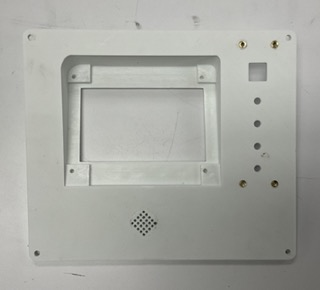
\includegraphics[width=\textwidth]{graphics/Empty Lid.jpeg}
            \caption{Heat Inserts In the Lid}
            \label{fig:Lid Heat Inserts}
        \end{subfigure}
        \begin{subfigure}{.45\textwidth}
            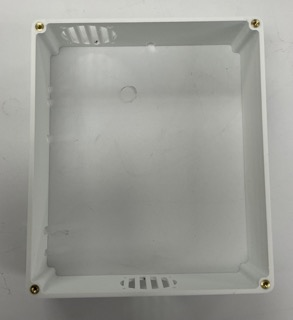
\includegraphics[width=\textwidth]{graphics/Enclosure Walls.jpeg}
            \caption{Heat Inserts In the Walls}
            \label{fig:Lid Heat Inserts 2}
        \end{subfigure}
    \end{figure}
\pagebreak
\subsection{Attaching Key Card Reader}
Due to the variance in screw hole placement on different brands of key card scanners, the holes must be manually marked and drilled for each assembly. First, place chosen scanner on a piece of paper and mark the screw hole placement by pushing a marker or pen through the paper and into the holes. Next, place the paper on the outside of the right enclosure wall (see photo) and mark the hole placement using the guide. Then drill out the holes with a bit corresponding with the size of the scanner's screws. 
Finally, screw the scanner into place on the outside of the enclosure walls with 3/8in 4/40 screws and with 2 washers on each screw, threading the screws from inside the wall through to the scanner.
\begin{figure}[H]
        \centering
        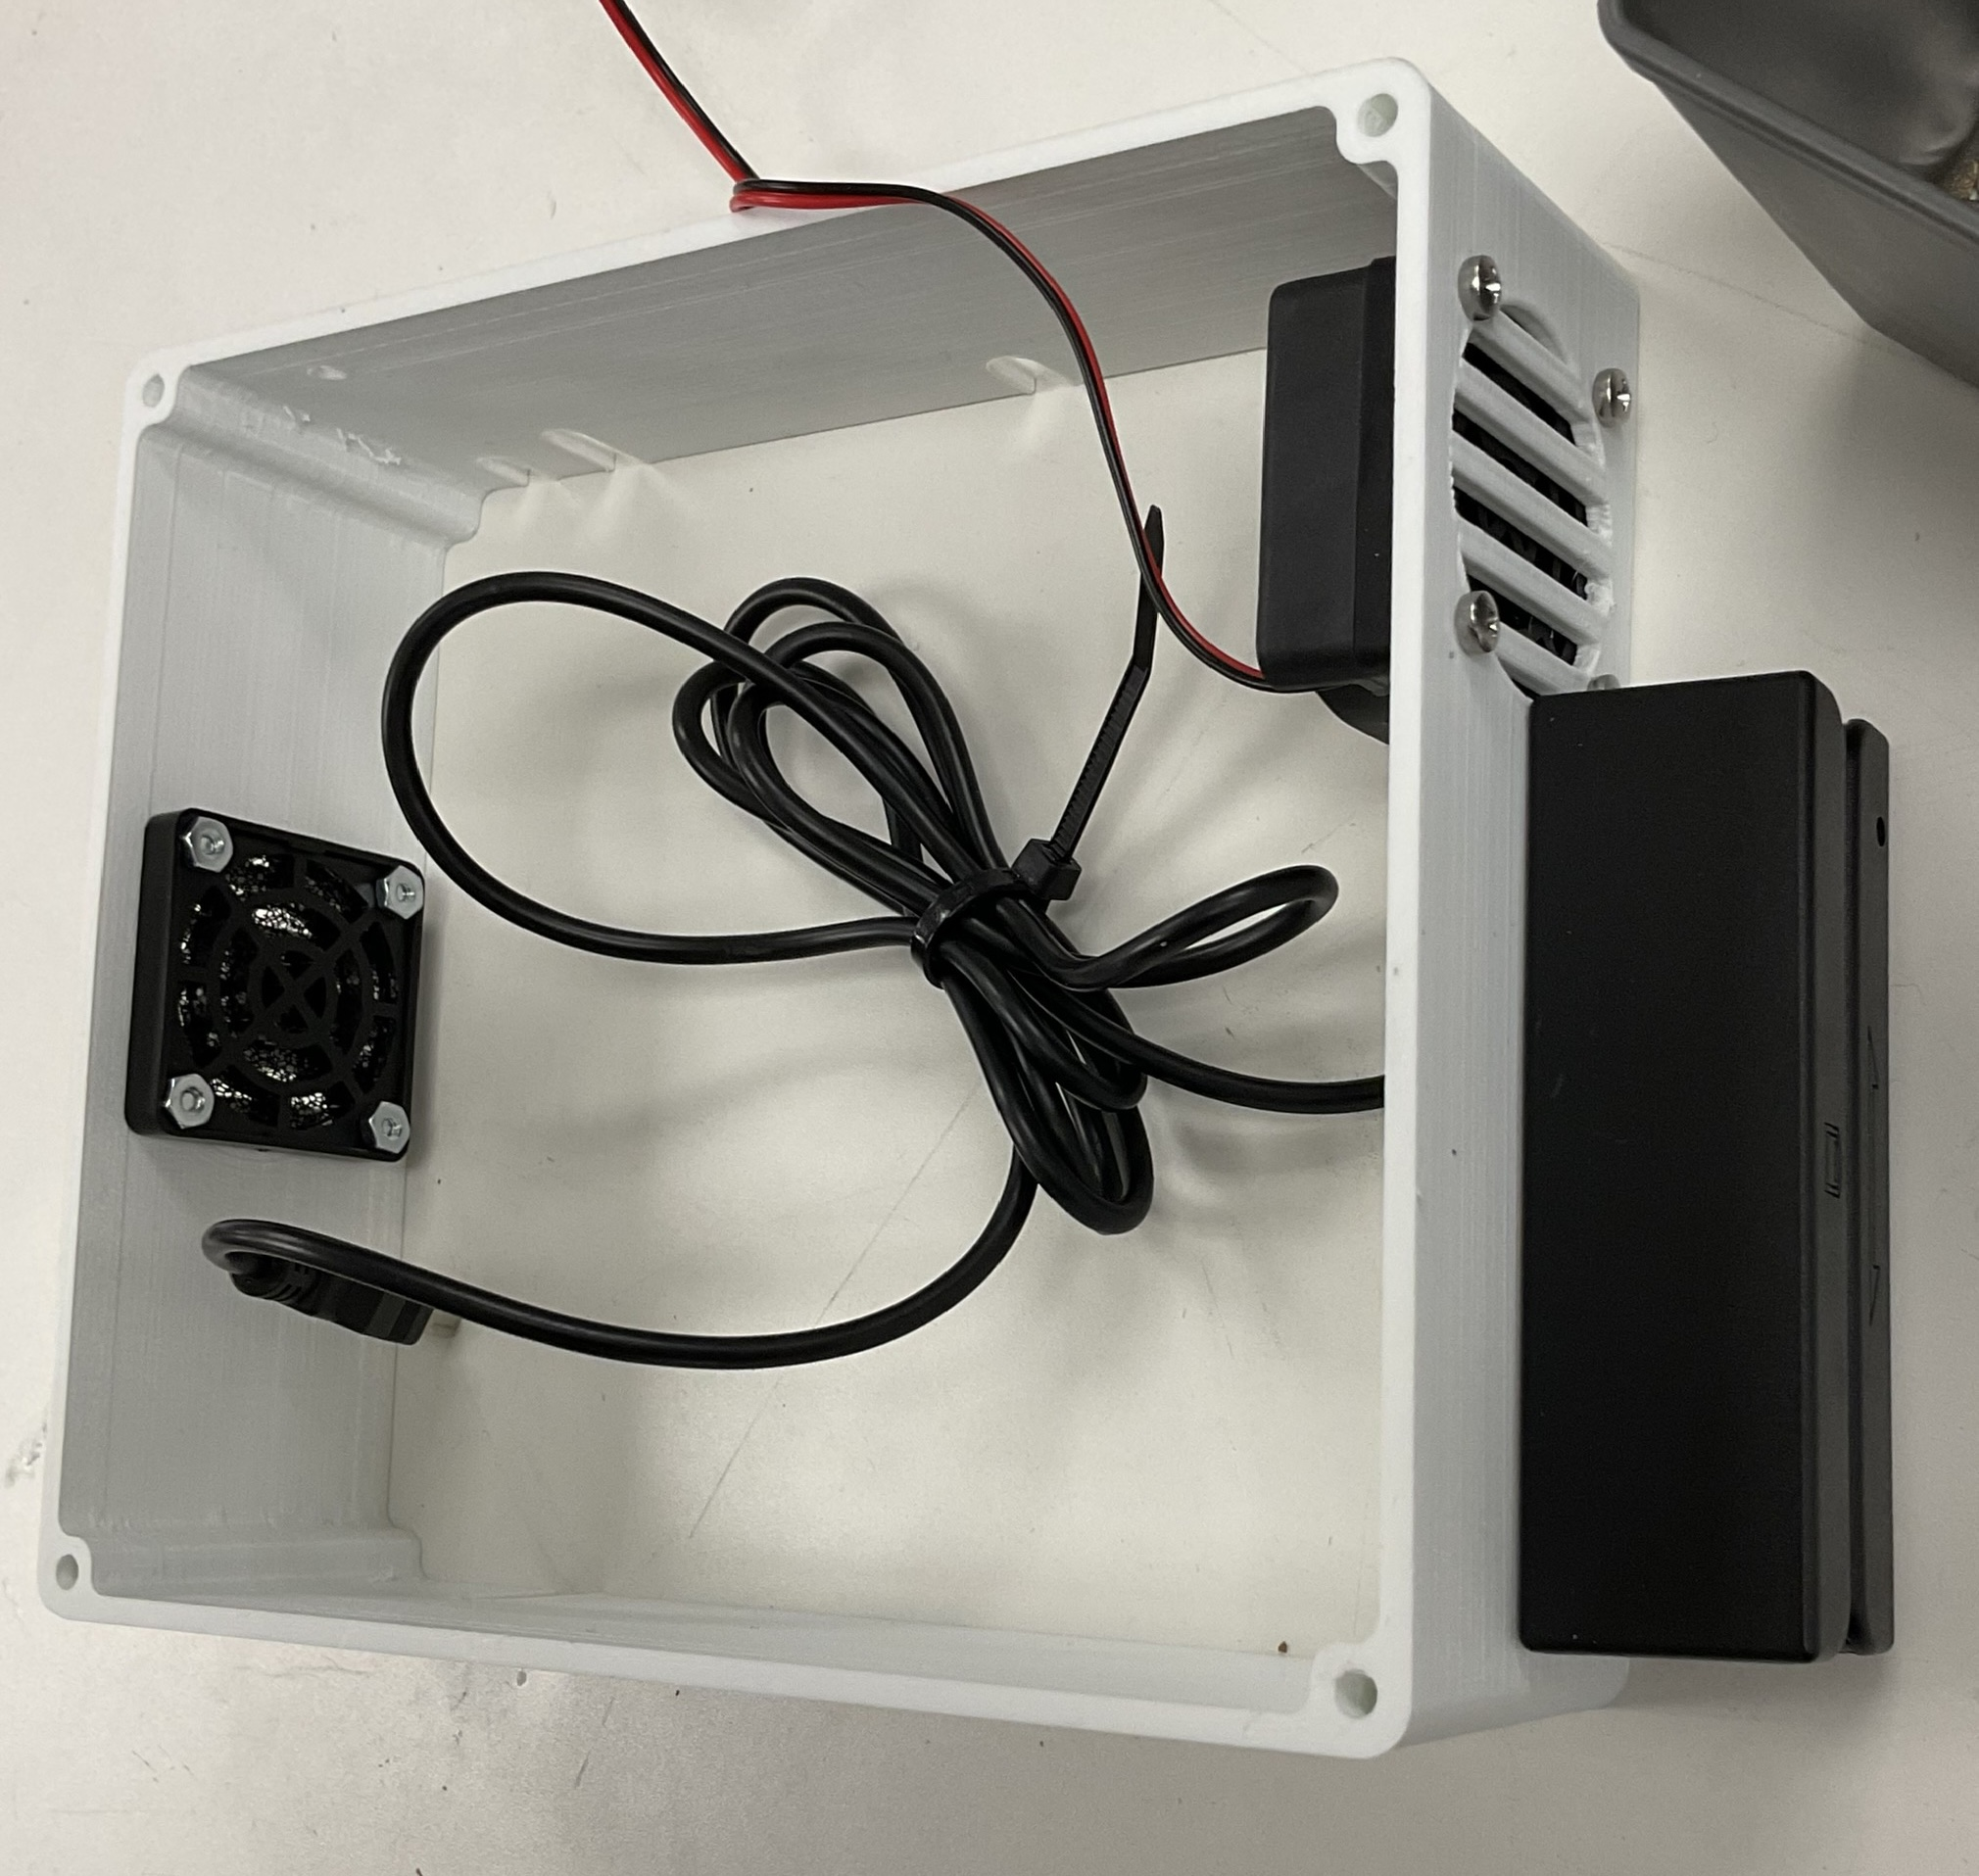
\includegraphics[width=.5\textwidth]{graphics/Scanner.jpg}
        \caption{Scanner Attached to Enclosure}
        \label{fig:Scanner}
    \end{figure}
\pagebreak
\subsection{Securing Internals}
The main PCB will be placed on top of the Raspberry Pi by connecting the headers, with metal standoffs in between, placed at each of the screw holes. The 12mm M2.5 screws go through the holes on the bottom of the case and into the threaded standoffs in between the boards. M2.5 are inserted through the top of the main PCB and into the standoffs to secure both boards. The vent filters and fans can be attached to either vent on the inside of the enclosure walls using 4/40 screws, inserting the screw from outside the walls, through the fan and/or filter, and using a nut to secure. Then the fan's cable can be connected to the main PCB. Finally, connect all cables to their correct ports, add strain relief with plastic zip ties, and wrap and secure the excess cable from the scanner.
    \begin{figure}[H]
        \centering
        \begin{subfigure}{.45\textwidth}
            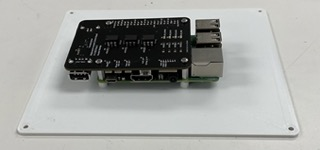
\includegraphics[width=\textwidth]{graphics/Bottom Internals.jpeg}
            \caption{Raspberry Pi and PCB Attached to Bottom Plate}
            \label{fig:Bottom Internals}
        \end{subfigure}
        \begin{subfigure}{.45\textwidth}
            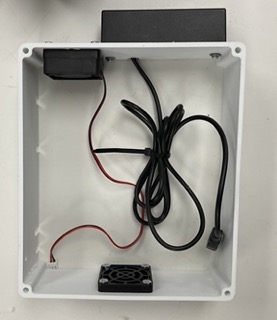
\includegraphics[width=\textwidth]{graphics/Fans.jpeg}
            \caption{Fans and Filters Attached to Walls}
            \label{fig:Bottom Internals 2}
        \end{subfigure}
    \end{figure}
\pagebreak
\subsection{Attaching Enclosure Walls}
After the cables have been connected to the correct ports and properly managed, the enclosure walls can be placed on top, ensuring the cables thread through the notches. Using the correct screws(3mm), the bottom enclosure plate can be secured to the walls by inserting the screws up through the bottom and into the walls.
\begin{figure}[H]
        \centering
        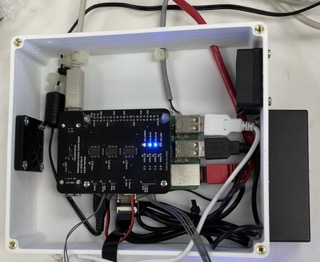
\includegraphics[width=.5\textwidth]{graphics/Internals Cables.jpeg}
        \caption{Cable Connections and Strain Relief}
        \label{fig:Cables}
    \end{figure}
\pagebreak
\subsection{Securing Lid and Connections}
The holes on the underside of the lid for the display must first be tapped using a 4-40 tap. Then the display can be screwed into place with the screws that come with them, ensuring the HDMI port is facing down. The secondary PCB can also be screwed into place on the underside of the lid with 4mm spacers in between the board and the lid to maintain the proper height. After both the HDMI cable and secondary board cable are connected to the main PCB and Raspberry Pi, the lid can be placed on top of the enclosure walls and secured in place with the 3mm security torx screws.
    \begin{figure}[H]
        \centering
        \begin{subfigure}{.45\textwidth}
            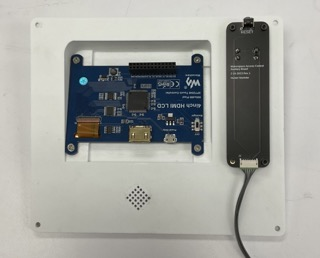
\includegraphics[width=\textwidth]{graphics/Lid Internals.jpeg}
            \caption{Display and Secondary PCB Attached to Lid}
            \label{fig:Lid Internals}
        \end{subfigure}
        \begin{subfigure}{.45\textwidth}
            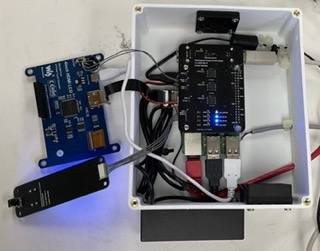
\includegraphics[width=\textwidth]{graphics/Internals Connections.jpeg}
            \caption{Cable Connections For All Internals}
            \label{fig:Final Cable Connections}
        \end{subfigure}
    \end{figure}
\subsection{Connecting to device}
Different devices will require different control methods. If it is a simple device that can just use USB then you just need to plug the USB line that plugs into the device into the controlling USB on the Main Board. If the device has a control line you will need the electrical schematic for that device and then find the door lines or another line that will pause the machine and then plug that line into our safety line control cable. If it is an AC-powered device then you will need to use a solid-state relay with a 3-5v control input voltage and then wire the power into that of whatever device you are trying to control as explained in \cref{sec: relay-controller}.

\pagebreak{}
\section{Database}
\newenvironment{databaseTable}
    { \begin{table}[H]
        \centering 
        \setlength{\tabcolsep}{8pt}
        \renewcommand{\arraystretch}{1.5} }
    { \end{table} }

\subsection{Implementation}
The databases are constructed using \lref{https://mariadb.org/}{MariaDB}.
The development version is constructed as a series of setup statements,
    collated from the \bashline{database} directory into \bashline{database_creation.sql} when \bashline{make} is run for the WebInterface respository.
These setup statements are run inside a docker compose project,
    using the docker image for MariaDB version 10.9.4.

\subsection{Databases and Access Control}
There are three databases, cross-referenced in views, to clearly define access rules.

\begin{databaseTable}
    \setlength{\tabcolsep}{24pt}
    \caption{Database Users}
    \label{table: database_users}
    \begin{tabular}{l l}
        \toprule
        User & Scope \\
        \midrule
        Controller\_Read & API commands retrieving data \\
        Controller\_Write & API commands writing data \\
        Admin\_Read & Web management reading system status \\
        Admin\_Write & Web management database modifications \\
        Root & Full permission base user \\
        \bottomrule
    \end{tabular}
\end{databaseTable}
\vspace{-1em}
\begin{table}[H]
    \centering
    \setlength{\tabcolsep}{18pt}
    \renewcommand{\arraystretch}{1.5}
    \caption{Overview of Databases}
    \label{table: database_overview}
    \begin{tabular}{l l l l}
        \toprule
        Database & Write Users & Read Users & Purpose \\
        \midrule
        Admin\_Utility & Admin & Admin & System Configuration \\
        Controller\_Utility & Controllers & Controllers & Configuration Data \\
        Logging & Controllers & Controllers, Admin & Usage Record \\
        \bottomrule
    \end{tabular}
\end{table}

\subsection{Table Layout}

\begin{databaseTable}
    \begin{tabular}{l c l}
        \multicolumn{3}{c}{\textbf{Admin\_Utility}} \\
        \toprule
        Table & Fields & Purpose \\
        \cmidrule(lr){1-3}
        assignments & controller\_id, device\_id & Associate controllers with devices \\
        blocked\_users & id, time, administrator, reason & Block trained users from system access \\
        devices & id, name, settings & Set configuration for each machine \\
        users & allowed\_device\_id & Give users access to specific machines \\
        \bottomrule \\
        \multicolumn{3}{c}{\textbf{Logging}} \\
        \toprule
        Table & Fields & Purpose \\
        \cmidrule(lr){1-3}
        log & time. controller\_id, device\_id, user, event & Record system usage and actions \\
        \bottomrule
    \end{tabular}
    \caption{Table Definitions}
    \label{table: table_defs}
\end{databaseTable}

\subsection{View Layout}

\begin{databaseTable}
    \setlength{\tabcolsep}{16pt}
    \begin{tabular}{l c l}
        \multicolumn{3}{c}{\textbf{Admin\_Utility}} \\
        \toprule
        View & Databases Used & Purpose \\
        \cmidrule(lr){1-3}
        auth\_failures & Logging, \hspace{0.1em} Admin\_Utility & Record of rejected accesses \\
        recent\_auth\_failures & Admin\_Utility & Rejected within past 24 hours \\
        repeat\_recent\_auth\_failures & Admin\_Utility & Times rejected in past 24 hours \\
        recent\_events & Logging, \hspace{0.1em} Admin\_Utility & Most recent event for per device \\
        \bottomrule \\
        \multicolumn{3}{c}{\textbf{Controller\_Utility}} \\
        \toprule
        View & Databases Used & Purpose \\
        \cmidrule(lr){1-3}
        allowed\_users & Logging, \hspace{0.1em} Admin\_Utility & User authorization testing \\
        pi\_settings & Admin\_Utility & Getting setup for assigned device \\
        \bottomrule
    \end{tabular}
    \caption{View Definitions}
    \label{table: view_defs}
\end{databaseTable}

\section{API}
\subsection{Implementation}
The API is built using \lref{https://laravel.com/}{Laravel}.
The development version is an image inside a docker-compose project,
    referencing a database container.
For deployment, the contents of \bashline{laravel_api/html} in the WebInterface repository can be copied to the target server.

\subsection{Authentication}
The API is meant exclusively for MakerSpace control unit access.
Units give their MAC address in a ``HTTP\_MAC'' header,
    and are only allowed to read and modify resources directly assigned to themselves.
Any unit not assigned to a MakerSpace device inside the database will not be given access.
If a machine's MAC address is compromised,
    the API access can be revoked by removing the MAC address from device assignments.

\subsection{GET Requests}
\begin{itemize}
    \item config
    \begin{itemize}
        \item Returns: JSON object of configuration settings
        \item Side effect: Logs that the device is alive
    \end{itemize}
\end{itemize}
\begin{itemize}
    \item auth\_user
    \begin{itemize}
        \item Input: JSON array of user IDs
        \item Returns: Boolean true or false for set of valid users
        \item Side effect: logs authentication request
    \end{itemize}
\end{itemize}
\begin{itemize}
    \item user\_admin
    \begin{itemize}
        \item Input: JSON array of user IDs
        \item Returns: Boolean true or false for set of admin users
        \item Side effect: logs authentication request
    \end{itemize}
\end{itemize}

\subsection{POST Requests}
\begin{itemize}
    \item log
    \begin{itemize}
        \item Input: JSON array of events
        \item Effect: adds given events to the controller's log
    \end{itemize}
\end{itemize}

\section{Admin Website}
\subsection{Implementation}
The website is constructed using \lref{https://www.php.net/}{PHP 8.1} on \lref{https://httpd.apache.org/}{Apache}, \lref{https://www.php.net/manual/en/book.mysqli.php}{mysqli}, and \lref{https://developers.google.com/chart/}{Google Charts} through \lref{https://developer.mozilla.org/en-US/docs/Web/JavaScript}{JavaScript}.
The development version is a docker image run inside the WebInterface docker compose project.
The files in \bashline{server/html} in the WebInterface repository can be copied to a host for deployment.

\subsection{Authentication}
All website pages are protected by Shibboleth (the development version uses generic .htaccess files).
Access to the database is controlled through locally stored credentials.
It is assumed that any user with access to the underlying environment,
    or can log into the webpage,
    should be given full control of the system and access to all secrets.
The two users constructed for interacting with the database are to protect against bugs,
    not to act as a protective measure.

\subsection{Functionality}
The website has full admin access to the database.
All actions are built upon a consistent main display page that is meant for desktop use.
Administrative changes (i.e. blocking a user) are performed through PHP form submissions.
Live data graphs are constructed through continuous JavaScript actions.
Any SQL commands outside of the prebuilt set should be performed with a separate MariaDB interactive client.

\section{Troubleshooting/Debugging}
\subsection{Boot Issues}
\begin{itemize}
    \item System takes a long time to boot
    \begin{itemize}
        \item Check that the SD card and power connector are properly seated.
        \item Check if the SD card has a slow read speed -- replace if so.
    \end{itemize}
    \item Error in Raspberry Pi boot process
    \begin{itemize}
        \item Check if the SD card is corrupted. Replace if it is.
        \item Flash SD card with a known working image.
    \end{itemize}
    \item System does not display UI fullscreen
    \begin{itemize}
        \item Change the sleep time in i3-config (inside the build directory) to be longer and re-flash
    \end{itemize}
\end{itemize}

\subsection{Communication Issues}
\begin{itemize}
    \item System does not connect to USB/Ethernet/etc.
    \begin{itemize}
        \item Re-seat all internal connectors.
        \item Verify cords are fully functional.
        \item Replace the Raspberry Pi.
    \end{itemize}
    \item System is not communicating with API.
    \begin{itemize}
        \item Check the system network connection.
        \item SSH into the system and run \bashline{getmac} to confirm the address was properly copied.
        \item Check for rejected communications in the admin interface, replace any incorrectly entered MAC address.
    \end{itemize}
    \item Admin Interface is not communicating with database.
    \begin{itemize}
        \item Check if the database is live.
        \item Log into the database and check for rejected connections.
        \item Update database user certifications.
    \end{itemize}
\end{itemize}

\subsection{Image Issues}
\begin{itemize}
    \item Image needs superuser permission to build/update/flash.
    \begin{itemize}
        \item Use a system where you have superuser access.
    \end{itemize}
    \item Image is corrupted on SD card.
    \begin{itemize}
        \item Mount the SD card data partition and run \bashline{fsck -fy FILESYSTEM}
        \item Decompress the latest image, loopback mount the data partition, and run \bashline{fsck -fy FILESYSTEM}
        \item If the image has no issues, but the SD card is corrupted after writing it again, discard the SD card.
        \item If the image has issues, go to an older image and check it. If it works, update the older image and reflash.
        \item If no older issues work, rebuild an image from scratch.
    \end{itemize}
\end{itemize}

\section{External Links}
\vspace*{-2em}
\printendnotes

\end{document}
